\documentclass[12px]{article}

\title{Lezione 15 Geometria I}
\date{2024-04-10}
\author{Federico De Sisti}

\usepackage{amsmath}
\usepackage{amsthm}
\usepackage{mdframed}
\usepackage{amssymb}
\usepackage{nicematrix}
\usepackage{amsfonts}
\usepackage{tcolorbox}
\tcbuselibrary{theorems}
\usepackage{xcolor}
\usepackage{cancel}

\newtheoremstyle{break}
  {1px}{1px}%
  {\itshape}{}%
  {\bfseries}{}%
  {\newline}{}%
\theoremstyle{break}
\newtheorem{theo}{Teorema}
\theoremstyle{break}
\newtheorem{lemma}{Lemma}
\theoremstyle{break}
\newtheorem{defin}{Definizione}
\theoremstyle{break}
\newtheorem{propo}{Proposizione}
\theoremstyle{break}
\newtheorem*{dimo}{Dimostrazione}
\theoremstyle{break}
\newtheorem*{es}{Esempio}

\newenvironment{dimo}
  {\begin{dimostrazione}}
  {\hfill\square\end{dimostrazione}}

\newenvironment{teo}
{\begin{mdframed}[linecolor=red, backgroundcolor=red!10]\begin{theo}}
  {\end{theo}\end{mdframed}}

\newenvironment{nome}
{\begin{mdframed}[linecolor=green, backgroundcolor=green!10]\begin{nomen}}
  {\end{nomen}\end{mdframed}}

\newenvironment{prop}
{\begin{mdframed}[linecolor=red, backgroundcolor=red!10]\begin{propo}}
  {\end{propo}\end{mdframed}}

\newenvironment{defi}
{\begin{mdframed}[linecolor=orange, backgroundcolor=orange!10]\begin{defin}}
  {\end{defin}\end{mdframed}}

\newenvironment{lemm}
{\begin{mdframed}[linecolor=red, backgroundcolor=red!10]\begin{lemma}}
  {\end{lemma}\end{mdframed}}

\newcommand{\icol}[1]{% inline column vector
  \left(\begin{smallmatrix}#1\end{smallmatrix}\right)%
}

\newcommand{\irow}[1]{% inline row vector
  \begin{smallmatrix}(#1)\end{smallmatrix}%
}

\newcommand{\matrice}[1]{% inline column vector
  \begin{pmatrix}#1\end{pmatrix}%
}

\newcommand{\C}{\mathbb{C}}
\newcommand{\K}{\mathbb{K}}
\newcommand{\R}{\mathbb{R}}


\begin{document}
	\maketitle
	\newpage
	\section{Ultima Parte teorica prima del compito}
	$O(2) = SO(2) \cup O(2)\setminus SO(2)$
	\[
		R_\theta = \matrice{cos\theta & -sin\theta\\ sin\theta& cos\theta}\ \ \ A_\theta = R_\theta A_\theta = \matrice{cos\theta& sin\theta\\ sin\theta & -cos\theta}
	.\] 
	\[
		R_\theta R_\varphi = R_{\theta + \varphi}
	.\] 
	\[
		A_\theta A_ \varphi = R_{\theta - \varphi}
	.\] 
	\begin{defi}[Riflessione]
		Isometria che fissa puntualmente una retta (detta asse della riflessione)
	\end{defi}
	$E$ piano euclideo
	$C\in E, r\subset E$ retta $\exists s,t$ rette passanti per $C$ tali che
	\[
	 R_{c,\theta} = \rho_r \circ\rho_s = \rho_t\circ\rho_r	.\] 
	"e viceversa"\\
	Possiamo fissare $c = 0 \ \ p_r = A_{o,\alpha}.$ Allora
	\[
		R_\theta = A_\alpha\circ A_{\alpha - \theta} = A_{\theta + \alpha}\circ A_\alpha
	.\] 
	dove $\rho_r = A_\alpha$ e $A_{\alpha - \theta} \equiv \rho_s$
\\
Il viceversa segue, sostituendo $c\equiv 0$, da $A_\alpha\circ A_\beta = R_{\alpha - \beta}$
 \[
	 R_{C,\theta}\circ R_{D,\varphi} \ \ \rightarrow \ \ \text{rotazione di angolo } \theta + \varphi \text{ Se } \theta + \varphi\neq 2k\pi,\ \ k\in \mathbb{Z}
.\] 
altrimenti è una traslazione (che è l'identità $ \LeftrightarrowC = D$)\\
Se $C = D$ chiaramente $R_{C,\theta}\circ R_{C, \varphi} = R_{C,\theta + \varphi}\\$
Se $C \neq D$ sia $r$ la retta per $C$ e $D$ Per la parte precedente possiamo scrivere
\[
	R_{C,\theta} = \rho_t\circ\rho_r, \ \ \ \ R_{D,\varphi} = \rho_r\circ\rho_s
.\] 
per certe rette $s,t$ 
\[
	T = R_{C,\theta}\circ R_{D,\varphi} = \rho_t\circ\rho_r\circ\rho_r\circ\rho_s
.\] 
Se $s,t$ sono incidenti allora per la parte precedente $T$ è una rotazione, altrimenti $s\parallel t$\\
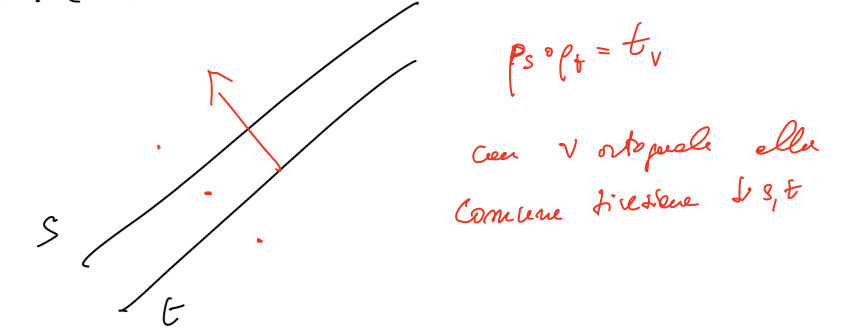
\includegraphics[scale=.4]{rette_parallele.png}\\
In coordinate rispetto ad un riferimetno cartesiano $Oe_1e_2$ Se $P\equiv\icol{x_1\\x_2}$ 
\[
	(R_{C,\theta}\circ R_{D,\varphi})(P) \ \ \ \text{ ha coordinate}
.\] 
\[
	R_\rho(R(x-d) + d-x) + x  
.\]
dove $c,d$ sono i vettori delle coordinate di $C,D $ rispettivamente\\
\begin{aligned}
	&\underline{R_{\theta + \varphi}(x - d)} + R_\theta(d-c) + c\\[-5px]
	&\hspace{-4px}\text{ parte lineare}
\end{aligend}\\[10px]
$T$ T è una translazione se e solo se $\theta + \varphi = 2k\pi, k\in\mathbb{Z}$ e in tal caso
\[
T(x) = x + R_\theta(d-c) = (d-c)
.\] 
che è l'identità se e solo se $d = c$ cioè $D=C$
\begin{defi}[Glissoriflessione]
	Una glissoriflessione è un'isometria di un piano euclideo ottenuta come composizione $t_v\circ\rho_r$ di una riflessione di asse $r$ con una traslazione $t_v\neq Id$ con $v\neq 0, v\parallel r$
\end{defi}
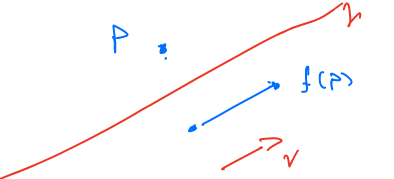
\includegraphics[scale=.4]{glissoriflessione.png}\\
\begin{teo}[Charles, 1831]
	Un'isometria di un piano euclideo che fissa un punto è una rotazione o una riflessione a seconda che sia diretta o inversa. Un'isometria senza punti fissi è una traslazione o una glissoriflessione a seconda che sia diretta o inversa
\end{teo}
\begin{dimo}
	Sia $f\in Isom(E)$\\ Se $f$ ha un punto fisso abbiamo già visto che $f$ è una rotazione se è diretta o una riflessione se $f$ è inversa\\
	se $f$ diretta priva di punti fissi. Allora anche $f^2$ non ha punti fissi, perché se $f^2(p) = p$ \\
	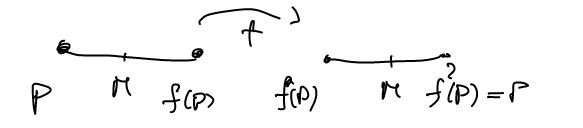
\includegraphics[scale=.4]{f_punti_fissi.png}\\
	Dunque $f(M) = M$ escluso.\\
	DIco che $p,f(p),f^2(p)$ che sono distinti per quanto abbiamo visto, sono allineati, Altrimneti  \textbf{Disegno TODO}\\
	\[
		d(P, f(p)) = d(f(p), f^2(p)) (\text{ poichè } f \text{ è un'isometria})
	.\] 
	\[
		d(Q,P) = d(Q,f(P)) = d(Q,f^2(P))
	.\] 
	Poiché $f$ preserva l'orientazione, il triangolo $QPf(P)$ viene trasformato in  $Q,f(P),f^2(P)$ da cui $f(Q) = Q$\\
	Dunque tutti i punti  $f^i(P), \ \ i\geq 0$ sono allineati, quindi se  $r$ è la retta che li contiene, $f$ agisce su $r$ come una traslazione.\\
	Poiché $f$ è diretta, $f$ agisce su tutto il piano come una traslazione.\\[10px]
	Sia ora $f$ inversa senza punti fissi,\\ Allora $f^2$ è diretta e come prima $f^2= t_v$ per qualche $v$\\
	Sia $P\in E$ un punto $r_0 = \overrightarrow{Pf^2(P)}, \ \ r_1 = \overrightarrow{f(P)f^2(P)}$ \\
	sono rette parallele che sono scambiate tra loro da $f$ \\
	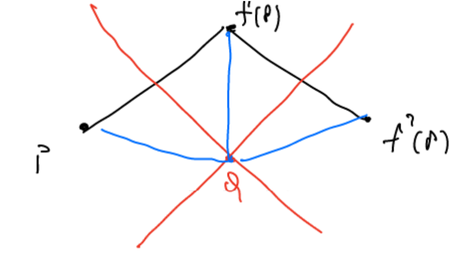
\includegraphics[scale=0.6]{batman.png}\\
	Sia $r$ la retta equidistante da $r_0$ e $r_1$.\\ Allora $f(r)\subseteq r  $ Ma $f^2 = t_v$ 
	$f|_r = t_{v/2}$\\
	Se ora consideriamo $t_{-v/2}\circ f$ \\questa è un'isometria inversa che fissa puntualmente $r$,\\ quindi è una riflessione che indichiamo con $\rho$. Dunque
	\[
		f = t_{v/2}\circ t_{-v/2}\circ f = t_{ v/2}\circ \rho
	.\] 
\end{dimo}
\subsection{Diagonalizzazione di operatori simmetrici}
\textbf{Ricorda}\\
$f\in End(V) $ diagonalizzabile se esiste una base di $V$ di autovettori di  $f\\ \Leftrightarrow A = [f]^B_B$ B base $\exists N\in GL(n,\mathbb{K}): N^{-1}AN$ è diagonale 
\begin{lemm}
	Il polinomio caratteristico di $A\in M_n(\mathbb{R})$ simmetrica ha solo radici reali
\end{lemm}
\begin{dimo}
	$A\in M_n(\mathbb{R}) \subseteq(\mathbb{C}) \ \ L_A : \mathbb{C}^n \rightarrow \C ^n.\\$
	Sia $\lambda\in \C$ un autovalore e $x\neq 0$ un corrispondente autovettore 
	\[
	Ax = \lambda x
	.\] 
	\[
		\overline{Ax} = \overline{\lambda x}
	.\] 
	\[
		A\overline{x} = \overline{\lambda}\overline{x}
	.\] 
	$\overline{x}^tAx = \overline{x}^t(Ax) = \overline{x}^t(\lambda x) = \lambda \overline{x}^t x\\
	\overline{x}^t A x = \overline{x}^t A^t x = (A\overline{x})^tx = (\overline{\lambda}\overline{x})^tx = \overline{\lambda}\overline{x}^tx$\\
	$\overline{x}^tx = \sum^n_{i=1}\overline{x}_ix_i$ $\leftarrow$ è un numero reale positivo poiché $x\neq 0$
	\[
		\lambda \overline{x}^tx = \overline{\lambda}\oveline{x}^tx \ \ \ \Rightarrow \ \ \ \lambda = \oveline{\lambda}
	.\] 
\end{dimo}
\begin{teo}[Teorema Spettrale]
	Sia $V$ uno spazio euclideo di dimensione finita e $T\in End(V)$ un operatore simmetrico, esiste una bas ortonormale di autovettori per $T$
\end{teo}
\begin{coro}
	Per ogni matrice reale simmetrica $A\in M_n(\R)$ esiste una matrice ortogonale $N\in O(n)$ tale che 
	 \[
		 N^{-1}AM = N^tAN \ \ \ \ \ \text{ è ortogonale}
	.\] 
\end{coro}
\begin{dimo}[Teorema]
	 Per induzione su $n = dim(V)$. Base $n = 1$ ovvia\\
	 Supponiamo $n = dim(v) \geq 2$. Poichè $T$ è simmetrico il polinomio caratteristico ha radici reali (per il lemma precedente) quindi $T$ ammette un autovalore $\lambda$ d sia $e_1$ il suo corrispondente autovettore di lunghezza $1$
	 \[
	 V = \R e_1\oplus(\R e_1)^\perp
	 .\] 
	 Chiamo $U \equiv (\R e_1)^\perp$ \\Dico che $T|_U :U \rightarrow$, per cui $T|_U\in End(U)$\\
	 Infatti, dimostro che $u\in U \rightarrow T(u)\in U$\\
\textbf{ipotesi: } $ \langle u, e_1 \rangle = 0$\\
\textbf{Tesi:} $ \langle Tu, e_1 \rangle  = \langle u, T^te_1 \rangle = \langle u, Te_1 \rangle = \langle u, \lambda e_1 \rangle  = \lambda \langle u, e_1 \rangle  = 0$\\
dove abbiamo usato la simmetria di T\\
Chiaramente $T|_U$ è simmetrico, quindi per induzione $U$ ha una base ortonormale di autovettori $\{e_2,\ldots,d_n\}$.\\
Ne segue che $\{e_1,\ldots,e_n\}$ è una base ortonormale di $V$ formata da autovettori per $T$
\end{dimo}
\end{document}
